\def\mytitle{MATRICES USING PYTHON}
\def\myauthor{Ballepu Dheeraj Kumar}
\def\contact{dheeraj.ballepu@gmail.com}
\def\mymodule{Future Wireless Communication (FWC)}
\documentclass[10pt, a4paper]{article}
\usepackage[a4paper,outer=1.5cm,inner=1.5cm,top=1.75cm,bottom=1.5cm]{geometry}
\twocolumn
\usepackage{graphicx}
\graphicspath{{./images/}}
\usepackage[colorlinks,linkcolor={black},citecolor={blue!80!black},urlcolor={blue!80!black}]{hyperref}
\usepackage[parfill]{parskip}
\usepackage{lmodern}
\usepackage{amsmath,amsfonts,amssymb,amsthm}
\usepackage{tikz}
	\usepackage{physics}
%\documentclass[tikz, border=2mm]{standalone}
\usepackage{karnaugh-map}
%\documentclass{article}
\usepackage{tabularx}
\usepackage{circuitikz}
\usetikzlibrary{calc}
\usepackage{amsmath}
\usepackage{amssymb}
\renewcommand*\familydefault{\sfdefault}
\usepackage{watermark}
\usepackage{lipsum}
\usepackage{xcolor}
\usepackage{listings}
\usepackage{float}
\usepackage{titlesec}
\providecommand{\norm}[1]{\left\lVert#1\right\rVert}
\providecommand{\sbrak}[1]{\ensuremath{{}\left[#1\right]}}
\providecommand{\lsbrak}[1]{\ensuremath{{}\left[#1\right.}}
\providecommand{\rsbrak}[1]{\ensuremath{{}\left.#1\right]}}
\providecommand{\brak}[1]{\ensuremath{\left(#1\right)}}
\providecommand{\lbrak}[1]{\ensuremath{\left(#1\right.}}
\providecommand{\rbrak}[1]{\ensuremath{\left.#1\right)}}
\providecommand{\cbrak}[1]{\ensuremath{\left\{#1\right\}}}
\providecommand{\lcbrak}[1]{\ensuremath{\left\{#1\right.}}
\providecommand{\rcbrak}[1]{\ensuremath{\left.#1\right\}}}
\newcommand{\myvec}[1]{\ensuremath{\begin{pmatrix}#1\end{pmatrix}}}
\let\vec\mathbf
\providecommand{\mtx}[1]{\mathbf{#1}}
\titlespacing{\subsection}{1pt}{\parskip}{3pt}
\titlespacing{\subsubsection}{0pt}{\parskip}{-\parskip}
\titlespacing{\paragraph}{0pt}{\parskip}{\parskip}
\newcommand{\figuremacro}[5]

\begin{document}

\title{\mytitle}
\author{\myauthor\hspace{1em}\\\contact\\FWC22008\hspace{6.5em}IITH\hspace{0.5em}\mymodule\hspace{6em}ASSIGN-4}
\date{}
	\maketitle
		
	\tableofcontents
\vspace{5mm}
   \section{Problem}
\paragraph{ ABCD is a rhombus.show that the diagonal AC bisects angle A as well as angle C and diagonal BD bisects angle B as well as angle D. }
   \section{Solution}
   \textbf{Theory:}\\

   Given  ABCD is a rhombus \\ 
  

\textbf{To Prove:} Diagonals bisects angles\\

In rhombus\\
 $\norm{\vec{A}-\vec{B}}$=$\norm{\vec{B}-\vec{C}}$=$\norm{\vec{C}-\vec{D}}$=$\norm{\vec{D}-\vec{A}}$\\
$\norm{\vec{C}-\vec{O}}$=$\norm{\vec{O}-\vec{A}}$\\
$\norm{\vec{B}-\vec{O}}$=$\norm{\vec{O}-\vec{D}}$\\



\vspace{2mm}
\textbf{Termux commands :}
\begin{lstlisting}
python3 rhombus1.py
\end{lstlisting}


The input parameters for this construction are 
\begin{center}
\begin{tabular}{|c|c|c|}
	\hline
	\textbf{Symbol}&\textbf{Value}&\textbf{Description}\\
	\hline
	%${\theta}$& $\pi/3$&$ \angle $DAB\\
	%\hline
	%${\theta 1}$& $\pi/6$&$ \angle $DAC\\    
	%\hline
	\textbf{O}&$\
	\begin{pmatrix}
		0 \\
		0 \\
	\end{pmatrix}$%
	&Point O\\
	\hline
	\textbf{Z1}&2
	&Point Z1\\
	\hline                         
	\textbf{Z2}&2
        &Point Z2\\
	
	\hline
\end{tabular}
\end{center}
\vspace{.25 cm}
\textbf{To Prove:}\\ 
$\angle$ BCA= $\angle$DCA \\ 
$\angle$ DAC= $\angle$BAD \\
\begin{align}
 \vec{P2} = \vec{C} - \vec{B}\\
 \vec{P3} = \vec{C} - \vec{D}\\
 \vec{P5} = \vec{C} - \vec{A}
	\end{align}
		
`Angle between vectors P2,P5 is given by \\
\begin{align}
\vec{\cos \theta} =\frac{\vec{(C-B)}^T  \vec{(C-A)}}{\norm{\vec{(C-B)}}\norm{\vec{(C-A)}}}
\end{align}
%\begin{align}
%	\norm{\vec{C-B+A-C}^2}
%\end{align}
%\begin{align}
%	\norm{\vec{(C-B)}^2}+\norm{\vec{(A-C)}^2}+2\vec{(C-B)}^T\vec{(A-C)}=\norm{\vec{(A-B)}^2}
%\end{align}
\vspace{3mm}\\
\begin{align}
 \vec{P5} = \vec{C} - \vec{A}\\
 \vec{P3} = \vec{C} - \vec{D}
	\end{align}
  %a1=A-B\\
  
 % a5=A-O\\  
  
 \vspace{3mm}
 `Angle between vectors P5,P3 is given by \\
 \begin{align}
\vec{\cos \theta_1} =\frac{\vec{(C-A)}^T  \vec{(C-D)}}{\norm{\vec{(C-A)}}\norm{\vec{(C-D)}}}
 \end{align}

 \begin{align}                                                \norm{\vec{C-B+A-C}}^2
 \end{align} 
 \begin{align}     
	 \norm{\vec{C-B}}^2+\norm{\vec{A-C}}^2+2\vec{(C-B)}^T\vec{(A-C)}=\norm{\vec{(A-B)}}^2
 \end{align}
\begin{align}
	\norm{\vec{C-A+D-C}}^2
\end{align} 
\begin{align}
	\norm{\vec{C-A}}^2+\norm{\vec{(D-C)}}^2+2\vec{(C-A)}^T\vec{(D-C)}=\norm{\vec{(D-A)}}^2
\end{align}
by using equations 9 and 11 we get\\
\begin{align}
\vec{(C-B)}^T\vec{(C-A)}=\vec{(C-A)}^T\vec{(C-D)}
\end{align}	
\begin{align}
cos\theta_1 =cos\theta
\end{align}
$\therefore$ diagonals of a rhombus bisects the angles\\

 \section{Construction}
 	\begin{center}
     Figure of Construction
 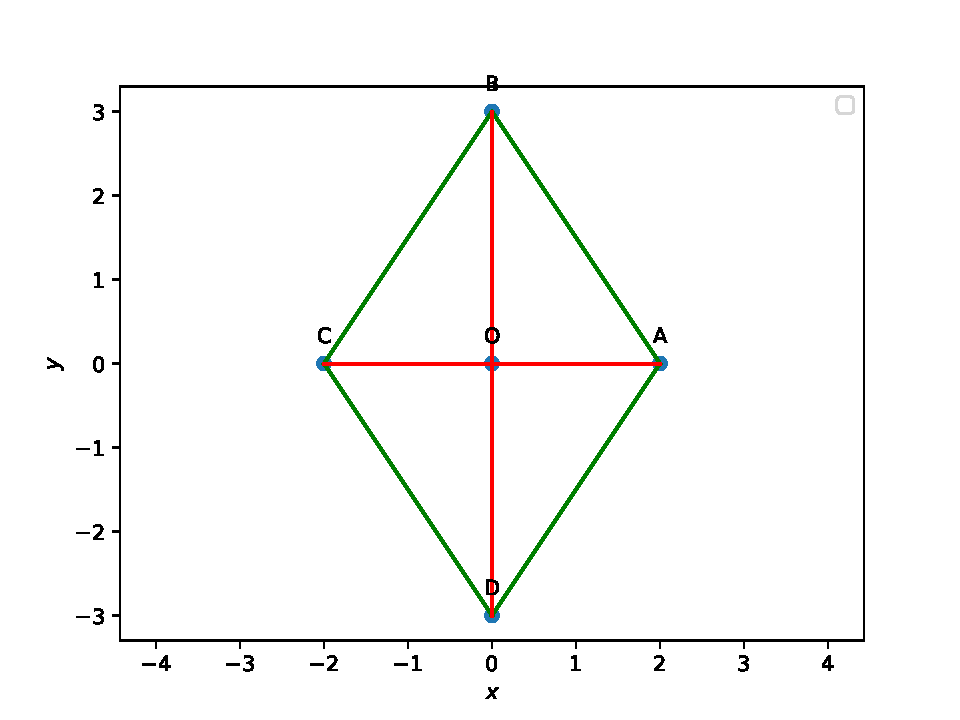
\includegraphics[scale=0.5]{fig/fig5.pdf} 
  	\end{center}
  	\vspace{1mm}
The below python code realizes the above construction:	\\
\url{https://github.com/ballepu1994/matricesline}
\bibliographystyle{ieeetr}
\end{document}

